\documentclass[11pt, aspectratio = 169]{beamer}

\usetheme[progressbar=frametitle]{metropolis}
\usepackage{appendixnumberbeamer}
\usepackage{booktabs}
\usepackage{amsmath}
\usepackage{mathtools}
\usepackage{bbm} % for math symbol \mathbbm
\usepackage{comment}
\usepackage{cancel}
\usepackage[scale=2]{ccicons}
\usepackage{pgfplots}
\usepgfplotslibrary{dateplot}
\usepackage{xspace}
\usepackage{hyperref}  
\usepackage{tikz}  
\usetikzlibrary{shapes,decorations,arrows,calc,arrows.meta,fit,positioning}
\tikzset{
    -Latex,auto,node distance =1 cm and 1 cm,semithick,
    state/.style ={ellipse, draw, minimum width = 0.7 cm},
    point/.style = {circle, draw, inner sep=0.04cm,fill,node contents={}},
    bidirected/.style={Latex-Latex,dashed},
    el/.style = {inner sep=2pt, align=left, sloped}
}
\usepackage{verbatim} 
\usepackage{listings}
\newcommand{\themename}{\textbf{\textsc{metropolis}}\xspace}
\definecolor{links}{HTML}{1B1B81}
\hypersetup{colorlinks,linkcolor=blue,urlcolor=blue}

% listings: To highlight code:
\usepackage{listings}
\lstset{
  language=R,
  basicstyle=\ttfamily\footnotesize,
  keywordstyle=\color{blue},
  commentstyle=\color{green!50!black},
  stringstyle=\color{red},
  frame=single,
  showstringspaces=false
}
\lstset{basicstyle=\ttfamily\footnotesize, frame=single}

\title{Applied Economics}
\subtitle{Panel Data Methods}
\author{Pello Aspuru}
\date{}
\institute{Winter 2025/26}
% \titlegraphic{\hfill\includegraphics[height=1.5cm]{logo.pdf}}
\setbeamercolor{normal text}{fg=black}
\setbeamercolor{block title}{fg=teal}
\setbeamercovered{transparent} % default faintness (~15%)

\let\svdescription\description
\let\svenddescription\enddescription
\renewenvironment{description}{%
  \svdescription%
  \let\svitem\item%
  \renewcommand\item[1][]{\svitem[\textcolor{\descriptioncolor}{##1}]}%
  }{
  \svenddescription%
  }
\newcommand\descriptioncolor{teal}

%\usepackage{Sweave}
\begin{document}
%\Sconcordance{concordance:AE_w9_panel.tex:AE_w9_panel.Rtex:%
1 47 1 1 0 458 1}

\maketitle

\begin{frame}{Plan for this Lecture}
\begin{enumerate}

\item What is Panel Data?

\item  Within and Between Variation

\item Panel Data Estimators
\begin{itemize}
\item Dummy Variable Estimator
\item First Differences
\item Within-Estimator 
\end{itemize}
\end{enumerate}
\end{frame}

\begin{frame}{Motivation}
Endogeneity due to OVB is a pervasive issue.

One approach to address it: instrumental variable regressions
\pause
Finding suitable instruments is very hard.

Today we consider an alternative approach to address certain forms of omitted variables: 
\textbf{panel data} allows to control for all \textit{time-invariant} unobservables.

\end{frame}

\section{What is Panel Data?}

\begin{frame}[fragile]{What is Panel Data?}

\begin{center}
    Does seatbelt use \alert{cause} a decrease in traffic fatalities?
\end{center}   
\begin{lstlisting}[language=R]
    df <- read.csv("./seatbelts.csv")
    head(df)
\end{lstlisting}
\pause
Panel data: Observe the same cross-sectional unit over multiple time periods 
\begin{itemize}
    \item \textit{cross-sectional unit} can be a person, company, city, \alert{state}, etc. ($i = 1,…n$) 
    \item \textit{time period} can be a month, a day, \alert{a year}, etc. ($t = 1,…,T$)
\end{itemize}

We denote a sample of panel observations as  $\{Y_{it}, \boldsymbol{X}_{it}\}$,  $i = 1, ... , n$, and $t = 1, ..., T$.
\end{frame}

\begin{frame}[fragile]{Balanced and Unbalance Panels}

\begin{itemize}
    \item \textbf{Balanced} panel: $\: \: \: \: \{Y_{it}, \boldsymbol{X}_{it}\}$ $i = 1, ..., n; t = 1, . . . , T$  \color{gray}[n x T observations in total] \color{black}
    \item \textbf{Unbalanced} panel: $\{Y_{it}, \boldsymbol{X}_{it}\}$, $i = 1, ..., n; t = \underline{t}_i . . . , \overline{t}_i$,
where $\underline{t}_i$ and $\overline{t}_i$ may vary across $i$. $\rightarrow$ we do not observe the same number of periods for each $i$.
    \pause
    \item[$\rightarrow$] Unbalancedness is prevalent, will abstract from this for the sake of exposition. 
\end{itemize}
\pause
\begin{center}
    Take a look to \texttt{df}. Is it balanced or unbalanced?
\end{center}

\end{frame}

\begin{comment}

\begin{frame}{(Unbalanced) Panel Data: Example}
\begin{columns}
    \begin{column}{.7\linewidth}
        \small \centering
    \begin{tabular}{l|l|r|r|r|l}
\toprule
state & year & fatalities & seatbelt & income & min age\\
\hline
\color{blue} AK & 1990 & 0.025 & 0.450 & 21073 & 16 \\
\color{blue}AK & 1991 & 0.025 & 0.660 & 21496& 16\\
\color{blue}AK & 1992 & 0.028 & 0.660 & 22073& 16\\
\color{blue}AK & 1993 & 0.030 & 0.690 & 22711& 16\\
\color{teal} AL & 1988 & 0.026 & 0.290 & 13288& 18\\
\color{teal}  AL & 1989 & 0.025 & 0.380 & 14266& 18\\
\color{teal} AL & 1990 & 0.026 & 0.440 & 15213& 18\\
\color{teal} AL & 1991 & 0.026 & 0.470 & 15895& 18\\
\color{teal} AL & 1992 & 0.023 & 0.580 & 16817& 18\\
\color{teal} AL & 1993 & 0.022 & 0.550 & 17398& 18\\
AR & 1988 & 0.032 & 0.301 & 12637& 21\\
AR & 1990 & 0.029 & 0.340 & 14025& 21\\
AR & 1991 & 0.028 & 0.520 & 14766& 21\\
&...&...&&\\
\bottomrule
\end{tabular}
    \end{column}

        \begin{column}{.353\linewidth}
        $i$ = state \\
        $t$ = year \\
        $Y_{it}$ = number of fatalities per \hspace*{+.69cm} million traffic miles  \\
        $X_{1it}$ = seat belt usage rate \\
         $X_{2it}$ = median income \\
         $X_{3it}$ = minimum drinking age

    \end{column}
\end{columns}

\end{frame}
\end{comment}

\begin{frame}{Panel Data - Features and Assumptions}
Focus on “large $n$, small $T$” panels.
\begin{itemize}
    \item many cross-sectional units $n$ (which may be randomly sampled) 
    \item observed for small number of time periods $T$ (which are typically ordered) \pause
    \item[$\rightarrow$] Small $n$, larg $T$ panels: time series econometrics, macroeconometrics. 
\end{itemize} 
\pause
\medskip 
Standard Assumptions:
\begin{itemize}
    \item cross-sectional units (e.g states) are \alert{randomly} sampled from a large population $\rightarrow$ i.i.d. across $i = 1, ... , n$.
    \item At the same time, we will \alert{not} make the i.i.d assumption within a unit $i$ across time (i.e., for a given unit $i$), as it is typically implausible in most settings.
    \small 
    \begin{itemize}
        \item example: state $i$ car fatalities in year $t$ and year $t+1$ 
    \end{itemize} 
\end{itemize}
\end{frame}

\begin{frame}[fragile]{Detour: \texttt{dplyr} Package for Data Manipulation}

\textbf{The Pipe Operator \texttt{\%>\%}} Reads as “\textit{and then}”
\vspace{-0.15cm}
\begin{itemize}
    \item Passes the left-hand side as the first argument to the function on the right.
\end{itemize}
\pause
\textbf{Core \texttt{dplyr} Verbs:}
\vspace{-0.15cm}
\begin{itemize}
    \item \texttt{arrange()} – sort rows
    \item \texttt{group\_by()} – apply operations within groups
    \item \texttt{summarise()} – compute summary statistics
    \item \texttt{mutate()} – create or transform variables
    \item Many other: \texttt{filter()}, \texttt{select()}, ...
\end{itemize}
\pause
Example: find average seatbelt use per state, save as \texttt{df\_average}:
\begin{lstlisting}[language=R]
    df_average <- df %>% group_by(state) 
                     %>% summarise(avg_usage = mean(seatbelt_usage))
\end{lstlisting}
\pause
\vspace{-0.2cm}
\begin{center}
    How many rows and columns will \texttt{df\_average} have? 
\end{center}
\end{frame}

\section{Within and Between Variation}


\begin{frame}[fragile]{Single Linear Regression - Pooled OLS}
Start from a single linear regression model of fatality rates $Y_{it}$ and seatbelt use $X_{1,it}$
\begin{align*}
   Y_{it} = \beta_0 + \beta_1 X_{1,it} + u_{it} , \quad \quad i = 1, ... , n; \quad \quad t = 1, ... , T. 
\end{align*}
Seatbelt use $X_{it}$ varies \alert{between} states and \alert{within} states.
\pause

\color{teal}\textbf{Pooled OLS} \color{black}
Estimate the parameters of the model by OLS
\begin{lstlisting}[language=R]
    pooled_slr <- lm(fatality_rate ~ seatbelt_usage, data = df) 
    coeftest(pooled_slr, vcov. = vcovHC(pooled_slr, "HC0"))
\end{lstlisting}
\pause
\begin{itemize}
\item Advantage: Slope parameter $\beta_1$ is estimated using \alert{between} and \alert{within} variation.
\item Disadvantage: Endogeneity is very likely $E[u_{it} X_{it}] \neq 0$
\end{itemize} 

\end{frame}

\begin{frame}[fragile]{Single Linear Regression Pooled OLS - First Look at Data}
    Plot the correlation between the main regressor and the outcome variable
    \begin{lstlisting}[language=R]
        scatter_1 <-
            ggplot(df, aes(x = seatbelt_usage, y = fatality_rate, 
                           color = state)) +
            geom_point(size = 3) + 
            geom_smooth(method = "lm", se = FALSE, color = "blue") + 
            labs(x = "Seatbelt Usage", y = "Fatality Rate") +
            theme_minimal() +
            theme(legend.position = "bottom")
    \end{lstlisting}
    \pause
    Save plot:
    \begin{lstlisting}[language=R]
        ggsave("./AE_week9_panel/scatterplot_1.pdf", 
                plot = scatter_1, width = 7, height = 5)
    \end{lstlisting}
\end{frame}

\begin{frame}[fragile]{Pooled OLS - First Look at Data}
    \only<1>{
    \begin{center}
        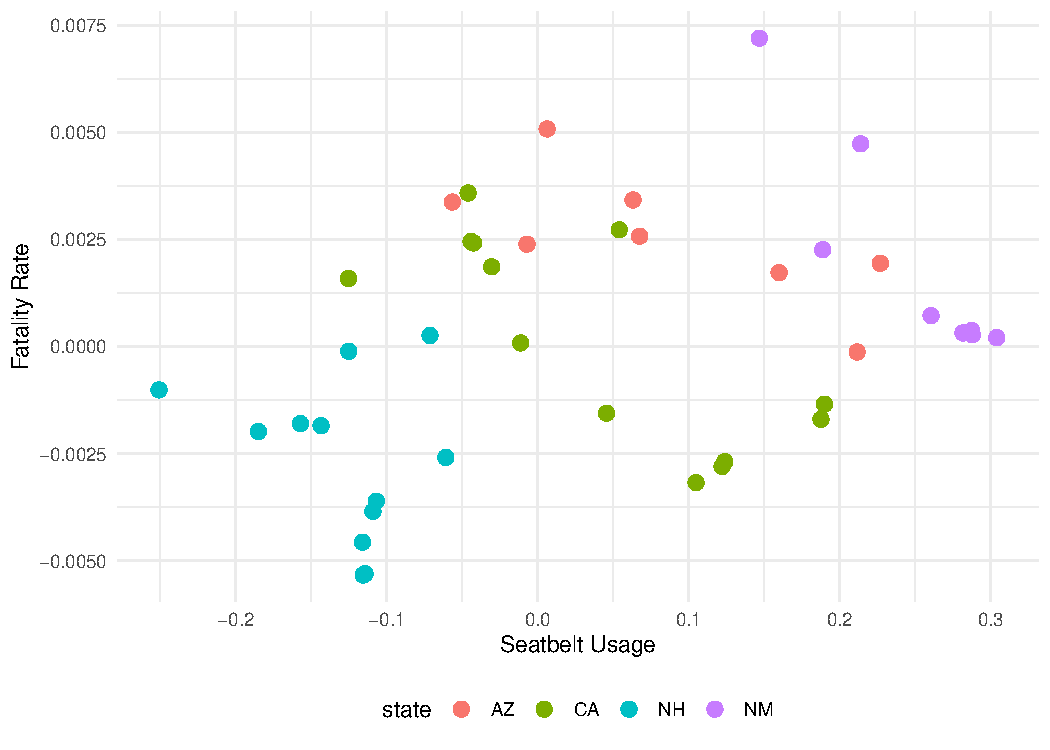
\includegraphics[height = 0.9\textheight]{scatterplot_0.pdf} 
    \end{center}}
    \only<2>{
    \begin{center}
        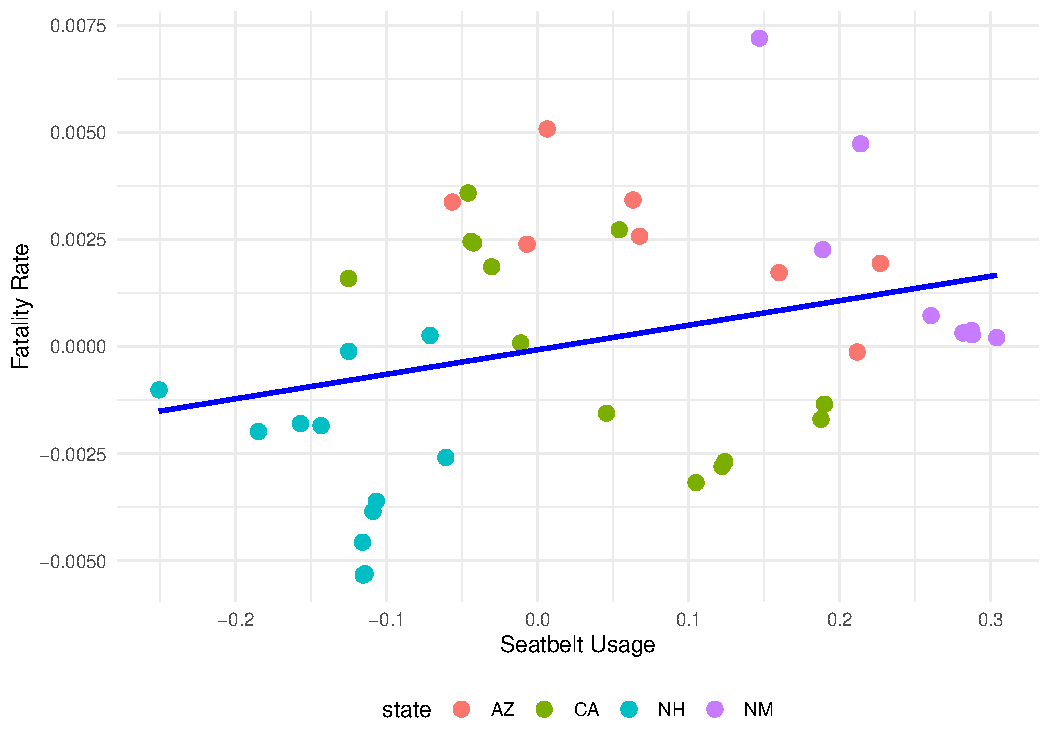
\includegraphics[height = 0.9\textheight]{scatterplot_1.pdf} 
    \end{center}}
\end{frame}

%\section{Within- vs. between-variation}

\begin{frame}[fragile]{Endogeneity}
    We can tame endogeneity with a pooled multiple linear regression that controls for mean state income $X_{2,it}$ and mean age $X_{3,it}$:
    \begin{align*}
    Y_{it} = \beta_0 + \beta_1 X_{1,it} + \beta_2 X_{2,it} + \beta_3 X_{3,it} + v_{it} , \quad \quad i = 1, ... , n; \quad \quad t = 1, ... , T. 
    \end{align*}
    \begin{lstlisting}[language=R]
    pooled_mlr <- lm(fatality_rate ~ seatbelt_usage + income + age, 
                     data = df) 
    coeftest(pooled_mlr, vcov. = vcovHC(pooled_mlr, "HC0"))
    \end{lstlisting}
    \pause
    \begin{itemize}
        \item Advantage: Slope parameters $\beta$ are estimated using \alert{between} and within variation.
        \item Disadvantage: \alert{Endogeneity} is very likely $E[v_{it} X_{it}] \neq 0$
        \item[$\rightarrow$] Previous advantages and disadvantages remain. 
    \end{itemize}
    \pause
    \begin{center}
        Panel Data Method intuition: \\
        sacrifice the \alert{between} variation in exchange of less \alert{endogeneity}.
    \end{center}
\end{frame}

\begin{frame}{Within- vs. between-variation}

Pooled OLS treats the whole data as one large (pooled) i.i.d. sample.
\vspace{-0.23cm}
\begin{itemize}
    \item often not justified as observations are not independent within units $i$ across $t$.
    \item moreover, it does not exploit the specific advantages of panel data!
\end{itemize}
\bigskip
\pause    
In a panel data set, we can decompose the total variation in our variables into

\begin{enumerate}
    \item \alert{within variation:} changes within each cross-sectional group $i$ over time.
    \begin{itemize}
        \item[$\rightarrow$] Used to estimate slope parameter $\beta_1$. 
    \end{itemize}
     \item \alert{between variation:} changes between cross-sectional groups
     \begin{itemize}
        \item[$\rightarrow$] Used to reduce endogeneity. 
    \end{itemize} 
\end{enumerate}

Example: seat belt usage rate varies \textit{between} states, and \textit{within} each state across years. \\
minimum drinking age only varies between states. It is \alert{time-invariant}.
\end{frame}


\begin{frame}{The Panel Model}

Key assumption: \textbf{decompose} unobserved error term $u_{it}$ into two:
\begin{itemize}
    \item time-invariant component \alert{$c_i$}: only varies between units $i$.
    \item idiosyncratic error term $\epsilon_{it}$ that varies between \textit{and} within unit $i$ over time.
\end{itemize}
\pause
The decomposition allows us to rewrite the single linear regression model as:
\begin{align*}
       Y_{it} = \beta_0 + \beta_1 X_{1,it} + \underbrace{\alert{c_i} + \epsilon_{it}}_{u_{it}} , i = 1, ... , n; t = 1, ... , T. 
\end{align*}
\pause 
Assuming that \alert{\textbf{$c_i$}} is potentially correlated with included regressors $\boldsymbol{X}_{it}$:  $Cov(\boldsymbol{X}_{it},\alert{c_i}) \neq 0 \: \Rightarrow E[\epsilon_{it}+\alert{c_i}|\boldsymbol{X}_{it}] \neq 0 \: \rightarrow$ endogeneity, bias in pooled OLS
\pause
\begin{center}
    Pooled OLS exogeneity $E[u_{it}|\boldsymbol{X_{it}}] = 0$ 
    $\; \rightarrow \;$ \pause Panel exogeneity $E[\epsilon_{it}|\boldsymbol{X_{it}}, \alert{c_i}] = 0$
\end{center}
\pause
\begin{center}
    We control for all \textbf{time-invariant} endogeneity
\end{center}
\end{frame}

\section{Panel Data Estimators}

\begin{frame}
    How do we estimate conrol for the time-invariant endogeneity \alert{$c_i$} ? \\ \pause 
    Three different ways to estimate the \textbf{panel model}:
    \begin{enumerate}
        \item The Dummy Variable Regression
        \item First Differences Estimator
        \item Within Transformation
    \end{enumerate}
\end{frame}

\begin{frame}[fragile]{Option 1: The Dummy Variable Regression}
Explicitly add $c_i$ to our regression by adding a \alert{dummy} for each cross-sectional unit $i$.\footnote{Note: we either have to omit one dummy, or the constant $\beta_0$} 
\vspace{-0.2cm}
\begin{align*}
       Y_{it} = \cancelto{0}{\beta_0} \; + \;\beta_1 X_{1,it} \; + \; \alert{\underbrace{\alpha_1 \mathbbm{1}\{state = 1\}}_{c_1}} \; + \; ... \; + \; \alert{\underbrace{\alpha_n \mathbbm{1}\{state = n\}}_{c_n}}
       \; + \; \epsilon_{it} %, \: \: i = 1, ... , n; t = 1, ... , T. 
\end{align*}
\pause
\vspace{-0.9cm}
\begin{itemize}
    \item $E[\alert{c_i}|X_{1,it}] = 0$ \textbf{no longer} required for exogeneity. Examples? \pause
    \item $E[\epsilon_{it}|X_{1,it}, \alert{c_i}] = 0$ still required for exogeneity.   Examples?
\end{itemize}
\pause
\vspace{0.2cm}
\begin{lstlisting}[language=R]
    panel_dummy <- lm(fatality_rate ~ 0 + factor(state) + 
                      seatbelt_usage, data = df)
\end{lstlisting}
\pause
\vspace{-0.2cm}
\begin{itemize}
    \item[$\rightarrow$] Which state has the largest $c_i$ ? 
\end{itemize}
\end{frame}

\begin{frame}{Discussion}
We can estimate the model with the cross-sectional-unit-dummies by  OLS to obtain $\hat{\boldsymbol{\beta}}$. \\
$\rightarrow$ OLS is unbiased if $E[\epsilon_{it}|\boldsymbol{X_{it}}, c_i] = 0$ (Assumption 4 for this model).

Because all time-invariant unobservables are eliminated from $\epsilon_{it}$, this is a much less strong assumption than $E[u_{it}|\boldsymbol{X_{it}}] = 0$.

Example: weather conditions much more likely to satisfy conditional mean independence than population's attitude towards seat belts.

When thinking about omitted variables that might be correlated with included regressors, we can ignore all time-invariant unobservables.  Every conceivable time-invariant variable is accounted for in our analyses!
\end{frame}

\begin{frame}{Interpretation}
    Pooled OLS: \\ Comparing seat belt usage rate and fatality rates \textit{across states and years}, we find that an increase in the seatbelt usage rate by 0.1 (10 percentage points) is associated with an \textit{increase} in the number of fatalities per million miles driven by .00057.  \color{gray} (=2.9\% of the sample mean).
\pause
\bigskip
\color{black}

Dummy variable estimation: \\ Comparing seat belt usage rate and fatality rates \textit{within states over time}, we find that an increase in the seat belt usage rate by .1 is associated with a \textit{decrease} in the number of fatalities per million miles driven by .0017.  \color{gray} (=8.6\% of the sample mean).

    
\end{frame}

\begin{frame}[fragile]{Illustrating the Panel Model}
    Use \texttt{dplyr} to generate an auxiliar dataset \texttt{pred\_df} fitting same $\beta_1$ within each state:
    \begin{lstlisting}[language=R]
        pred_df <- df %>%
        group_by(state) %>%
        summarize(
            seatbelt_usage = seq(min(seatbelt_usage), 
                                max(seatbelt_usage), 
                                length.out = 100),
            .groups = "drop" # remove previous grouping.
        )
        pred_df$pred <- predict(panel_dummy, newdata = pred_df)
    \end{lstlisting}
\end{frame}

\begin{frame}[fragile]{Illustrating the Panel Model}
    Use \texttt{ggplot2} to generate scatterplot \texttt{scatter\_2}:
    \begin{lstlisting}[language=R]
        scatter_2 <-
        ggplot(df, aes(x = seatbelt_usage, y = fatality_rate, 
               color = state)) +
        geom_point(size = 3) +
        geom_line(data = pred_df, aes(y = pred), linewidth = 1) +
        labs(x = "Seatbelt Usage (%)", y = "Fatality Rate") +
        theme_minimal() +
        theme(legend.position = "bottom")
    \end{lstlisting}
\end{frame}

\begin{frame}{Pooled OLS - Scatterplot}
    \only<1>{
    \begin{center}
        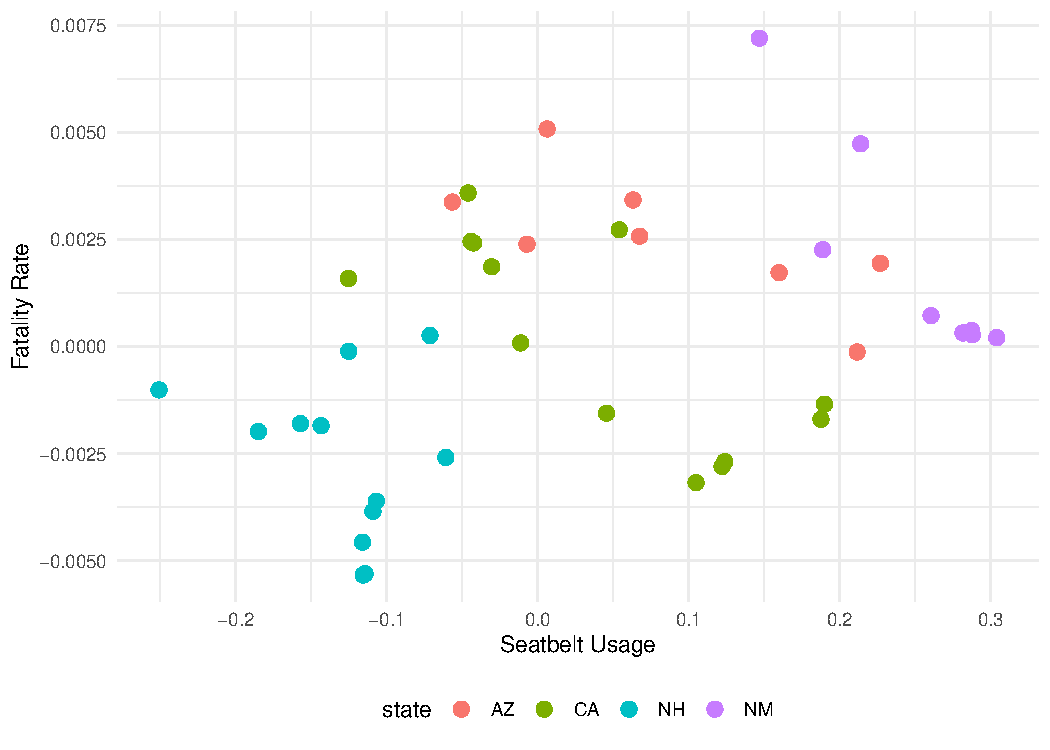
\includegraphics[height = 0.9\textheight]{scatterplot_0.pdf} 
    \end{center}}
    \only<2>{
    \begin{center}
        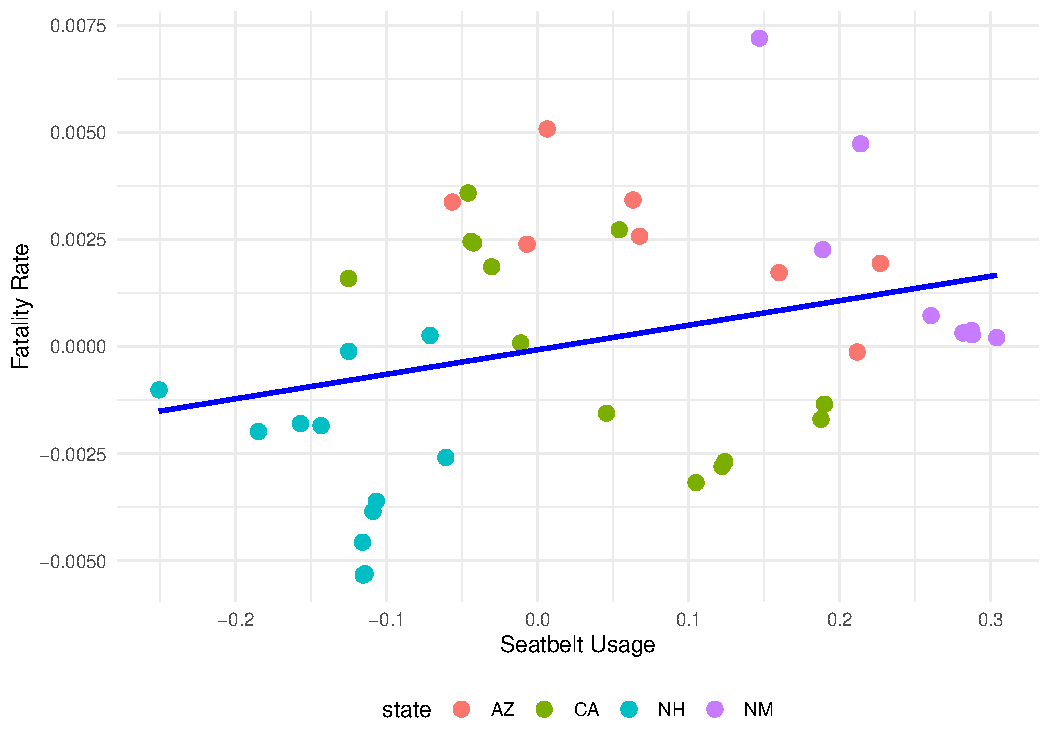
\includegraphics[height = 0.9\textheight]{scatterplot_1.pdf} 
    \end{center}}
\end{frame}

\begin{frame}{Panel Model - Scatterplot}
    \begin{center}
        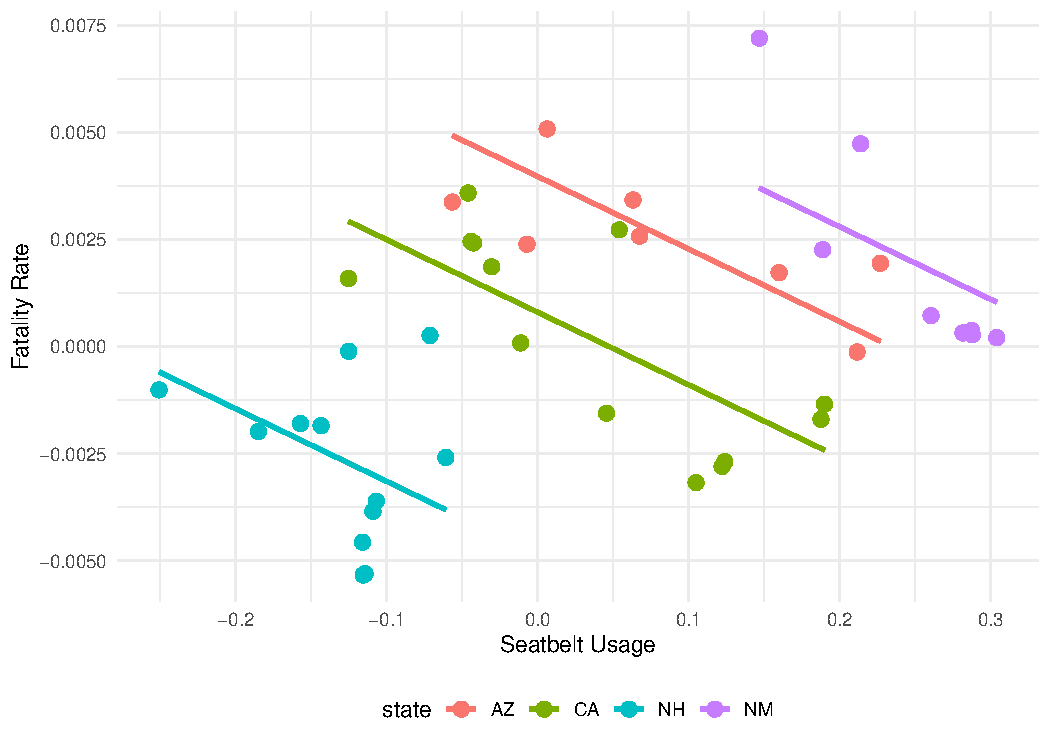
\includegraphics[height = 0.9\textheight]{scatterplot_2.pdf} 
    \end{center}
\end{frame}


\begin{comment}


\begin{frame}{Another Example}
Climate change literature: how do rising temperatures affect human health and productivity?

Say we are interested in the effect of outdoor temperature ($X_{it}$) on exam performance ($Y_{it}$) among students in Italy.

We have a \textbf{panel} of students $i = 1,...,n$ all across the country for multiple exams taken at dates $t = 1,...,T$.

Just regressing $Y_{it}$ on $X_{it}$ (pooled OLS) might yield biased estimates, e.g. if students in the warmer South study harder because of bad economic prospects in the South. 

$\rightarrow$ $X_{it}$ correlated with $u_{it}$ (e.g. effort)
\end{frame}

\begin{frame}{Another Example}
\begin{align*}
Y_{it} 
&= \boldsymbol{X}_{it} \boldsymbol{\beta}
   + \color{blue}
     \underbrace{\alpha_1 \mathbbm{1}\{ \text{student} = 1 \}}_{c_1}
     + \cdots
     + \underbrace{\alpha_n \mathbbm{1}\{ \text{student} = n \}}_{c_n}
     \color{black}
   + \epsilon_{it}, \\
& \qquad i = 1, \ldots, n; \quad t = 1, \ldots, T.
\end{align*}

Dummy-variable regression allows us to control for all time-invariant unobservables $c_i$,  
such as overall student effort or ability.

Effect of temperature is estimated from variation for each specific student over exam dates  
(within-student variation).
\end{frame}

\end{comment}


\begin{frame}{Option 2: First-Differences Estimator}

If $T = 2$, an alternative to the dummy variable approach is first-differencing:

Consider a generic MLR model for two time periods:
\begin{align*}
    Y_{i, t=1}& = \boldsymbol{X}'_{i, t=1}\boldsymbol{\beta} + c_i + \epsilon_{i, t=1}  \text{ and  } \\
Y_{i, t=2} &= \boldsymbol{X}'_{i, t=2}\boldsymbol{\beta} + c_i + \epsilon_{i, t=2}   
\end{align*}
\pause
Differencing yields: 
\begin{align*}
Y_{i, t=2} \;– \; Y_{i, t=1} &= (\boldsymbol{X}'_{i, t=2} - \boldsymbol{X}'_{i, t=1}) \boldsymbol{\beta} + \alert{(c_i – c_i)} + (\epsilon_{i, t=2} – \epsilon_{i, t=1}) \\
\text{ or: } \Delta Y_i &= \Delta \boldsymbol{X}_{i} \boldsymbol{\beta} + \Delta\epsilon_i
\end{align*}
\pause
$\rightarrow$ The unobserved heterogeneity \alert{$c_i$} drops out! (and also $\beta_0$)

\pause 
This is our “estimating equation”. \\
We can estimate $\boldsymbol{\beta}$ by OLS by regressing $\Delta Y_i$ on $\Delta \boldsymbol{X}_i$. \\
The estimator is unbiased if $E[\Delta\epsilon_i|\Delta \boldsymbol{X}_{i}] = 0$ (MLR.4 for this model).
\end{frame}


\begin{frame}[fragile]{Option 3: Within Transformation}
%Option 3 The most common estimation approach is the \textit{within-transformation}.
\begin{enumerate}
    \item For all variables in your model, compute the \textbf{time-mean} for each unit $i$:
    \[
    \overline{Y_{i}} = \frac{1}{T} \sum_{t=1}^T Y_{it}, 
    \qquad 
    \overline{X}_{1i} = \frac{1}{T} \sum_{t=1}^T X_{1it} \quad \cdots \quad \alert{\overline{c_{i}} = c_i}
    \]
    %\item[$\rightarrow$] Note that  \alert{$\overline{c_{i}} = c_i$}
    \pause
    \item Deduct the time means from the actual values.  
    Obtain \textit{demeaned} variables:  
    \[\quad (Y_{it}-\overline{Y_{i}}),\quad (X_{1it}-\overline{X}_{1i}),\quad \ldots,\quad (X_{kit}-\overline{X}_{ki}), \quad \alert{(c_i - \overline{c_{i}})} \]
\end{enumerate}
\pause
Use \texttt{dplyr} to generate a demeaned variable dataset \texttt{df\_demeaned}:
\begin{lstlisting}[language=R]
df_demeaned <- df %>%
group_by(state) %>%
mutate(fatality_rate_dm   = fatality_rate - mean(fatality_rate),
       seatbelt_usage_dm  = seatbelt_usage - mean(seatbelt_usage)) %>%
ungroup()
\end{lstlisting}
\end{frame}

\begin{frame}[fragile]{Option 3: Within Transformation}
\textit{Demeaned} regression Model:
\begin{align*}
Y_{it}-\overline{Y}_{i} 
&= (\beta_0 - \beta_0)
  + \beta_1(X_{1it}-\overline{X}_{1i})
  + \cdots
  + \beta_k(X_{kit}-\overline{X}_{ki})
  + \alert{(c_i - \overline{c_i})}
  + (\epsilon_{it}-\overline{\epsilon}_i) \\
&= \beta_1(X_{1it}-\overline{X}_{1i})
  + \cdots
  + \beta_k(X_{kit}-\overline{X}_{ki})
  + (\epsilon_{it}-\overline{\epsilon}_i)
\end{align*}
\vspace{-1cm}
\begin{itemize}
    \item \alert{$c_i$} drops out because there is no \textit{within-variation} in $c_i$!
    \item Again, we can estimate this “demeaned equation” by OLS.
\end{itemize}
\pause
\begin{lstlisting}[language=R]
    panel_within_manual <- lm(fatality_rate_dm ~ 0 + seatbelt_usage_dm, 
                              data = df_demeaned)
    coeftest(panel_within_manual, 
             vcov. = vcovHC(panel_within_manual, "HC0"))
\end{lstlisting}
\end{frame}

\begin{frame}[fragile]{Within Estimator with \texttt{fixest}}
We can directly implement the within-estimator in R using the command
\alert{\texttt{feols}} from the package \alert{\texttt{fixest}}.
\pause
\begin{lstlisting}[language=R]
panel_within_fixest <- feols(fatality_rate ~ seatbelt_usage | state, 
                             data = df)
coeftest(panel_within_fixest, 
         vcov. = vcovHC(panel_within_fixest, "HC0"))
\end{lstlisting}
\end{frame}

\begin{frame}{Limitations of Panel Data Estimators}

Recall that, unlike pooled OLS, Panel Data models exploit only \textit{within-}variation for each unit $i$, i.e. \textbf{deviations from the unit-specific mean}. \pause
\begin{itemize}
    \item \alert{We cannot include time-invariant regressors} when using these estimators. 
    \begin{itemize}
        \item They would drop out, because they are absorbed by the individual fixed effect.
        \item In our example, we could not include a maximum speed control, right?
    \end{itemize} \pause
    \item For setups with little within group time-variation, we may \alert{not have enough variation} to estimate slope parameters.
\end{itemize}
\end{frame}

\begin{frame}{One More Thing...}

% ----- EQUATION AREA (fixed height) -----
\begin{minipage}[c][0.15\textheight][c]{\textwidth}
    \only<1>{
        \[
        Y_{it} = \beta_0 + \beta_1 X_{1,it} + u_{it},
        \quad i = 1,\ldots,n; \quad t = 1,\ldots,T.
        \]
    }

    \only<2->{
        \[
        Y_{it}-\overline{Y}_{i} 
        = \beta_1(X_{1it}-\overline{X}_{1i})
        %+ \alert{(c_i - \overline{c_i})}
        + (\epsilon_{it}-\overline{\epsilon}_i)
        \]
    }
\end{minipage}
\vspace{-1cm}
% ----- FIGURE AREA (fixed height) -----
\begin{minipage}[c][0.8\textheight][c]{\textwidth}
    \centering
    \only<1>{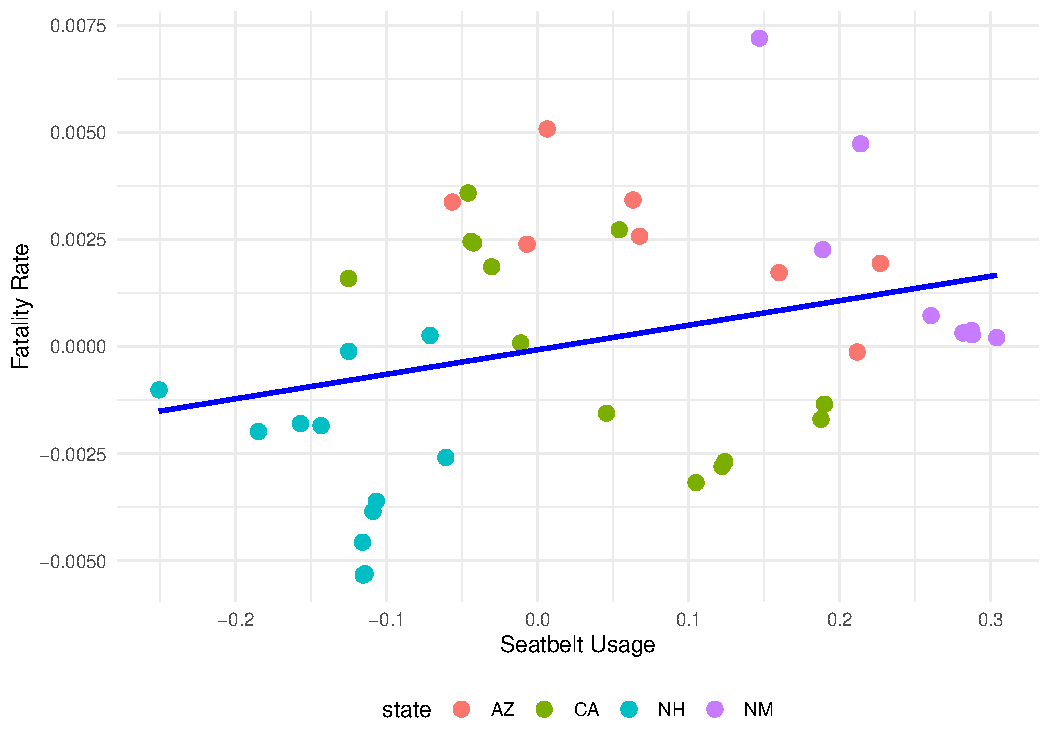
\includegraphics[height=0.7\textheight]{scatterplot_1.pdf}}
    \only<2>{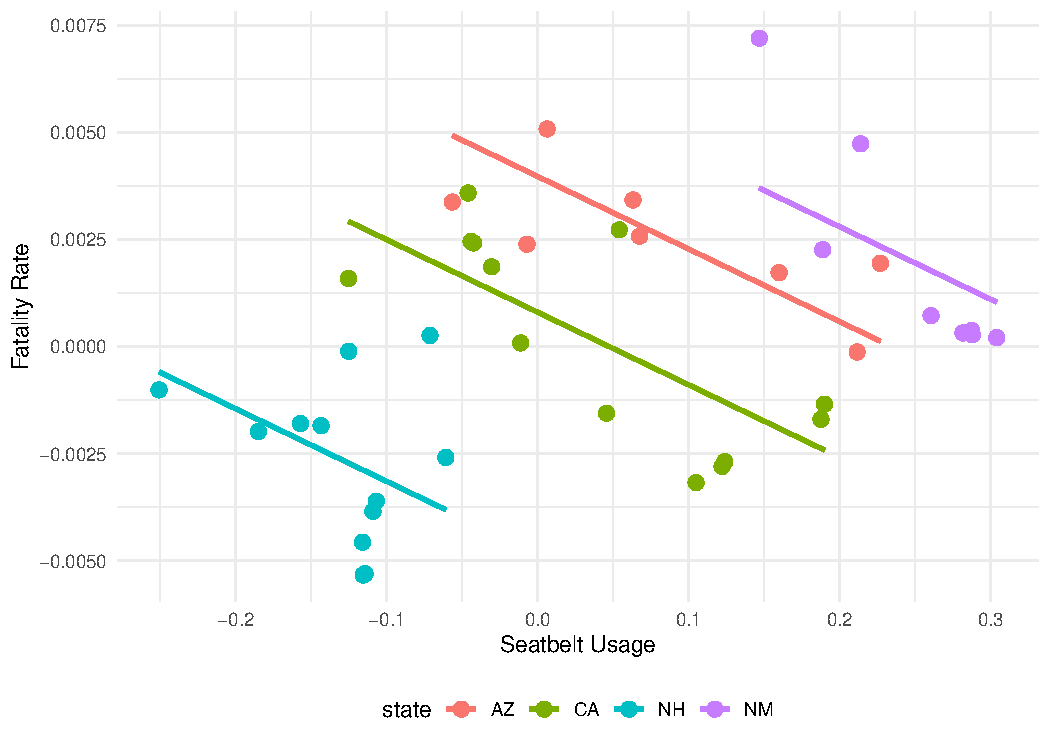
\includegraphics[height=0.7\textheight]{scatterplot_2.pdf}}
    \only<3>{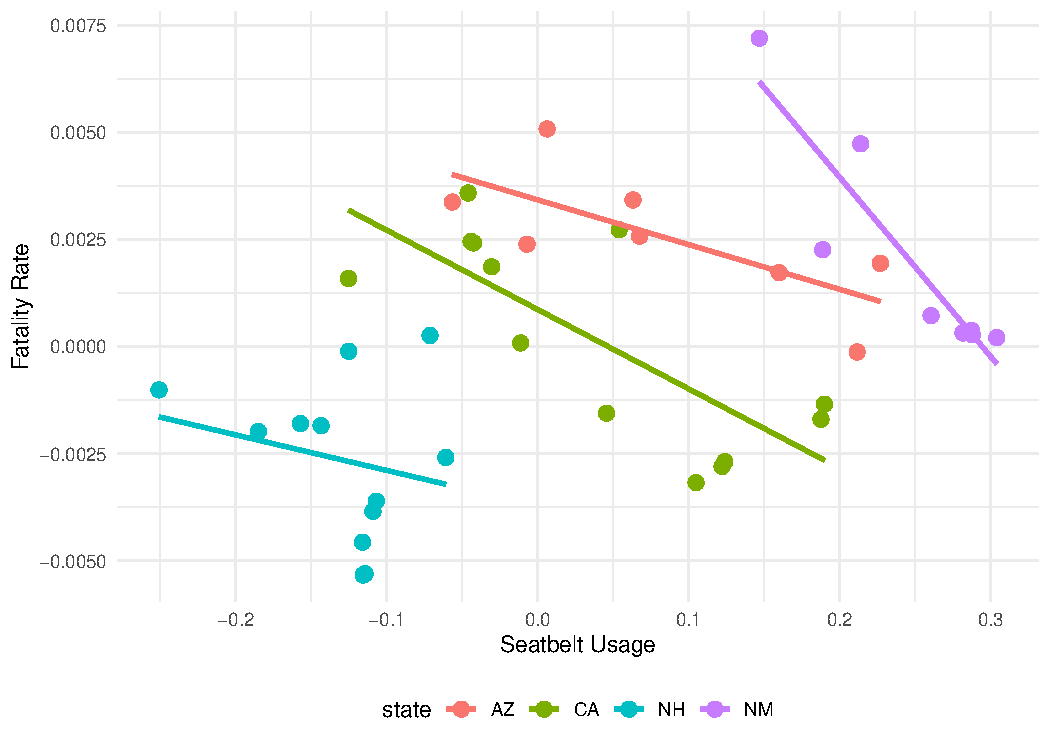
\includegraphics[height=0.7\textheight]{scatterplot_3.pdf}}
\end{minipage}

\end{frame}


\end{document}







